\chapter{Android Platform}
\label{chap:Android Platform}

In this chapter, we explore the workings of the Android platform, how each layer in the stack contributes to Android security and safe communication between processes.  We use the first chapter from the Nikolay Elenkov book `Android Security Internals' \cite{AndroidSecurityInternals} as our source and guidance.

\begin{figure}[h]
  \centering
  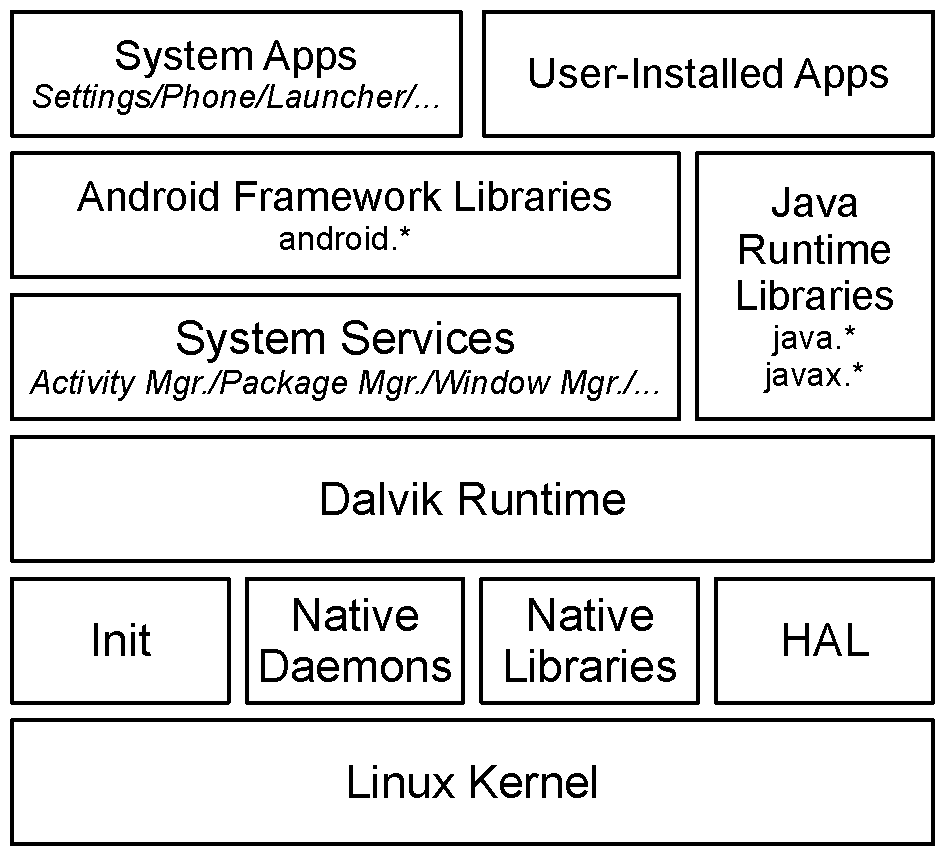
\includegraphics[width=0.5\textwidth]{graphics/AndroidStack.pdf}
  \caption{The Android architecture}
  \label{fig:AndroidStack}
\end{figure}

\section{Linux}
\label{sec:Linux}

At its core, Android is built on the Linux kernel with some modifications specific to Android.  The standard security mechanisms provided by Linux enforce process isolation through sandboxing and user-based file access permissions.  Android adds two more features to the standard Linux kernel.  First, a feature called paranoid networking forces processes to have permission to use sockets. The second is an IPC system called Binder that underpins all IPC methods in Android.  We describe Binder in more detail in section \ref{sec:IPC} and permissions in \ref{sec:Permissions}.

Above the kernel layer is the Init binary, native daemons, native libraries, and a hardware abstraction layer (HAL).  The Init binary contains the first process started by Linux, the zygote process, and native daemons run in the background providing services and functionality.  The HAL is a daemon that maintains a realtime database of devices connected to the system and provides an API that applications can use to discover, monitor and invoke operations on devices. The Linux native libraries are code collections, such as the standard C routines or encryption functions, for application programmers.

\subsection{Sandboxing}
\label{sec:Sandboxing}

The sandboxing feature of Linux gives each installed android package a unique userId.  A Linux process can only execute code with the same userId, so different packages get forced to run in different processes.  Linux uses memory management to separate processes into their own address spaces.  By doing so, a process is unable to reference other processes address space.  They cannot corrupt each other's memory, read, write or in any way communicate with each other directly via memory.  They are also unable to reference memory owned by operating system processes that run in protected mode.  Thus, they cannot insert code into the operating systems memory space to execute it in protected mode. 
  
\subsection{FileAccessPermissions}
\label{sec:FileAccessPermissions}  

The second feature provided by the Linux kernel is that of file access permissions.  Files are associated with an owner's userId (UID) and a groupId (GID) along with three tuples of read, write, execute permissions.  The first tuple is the owner's permission, the second is the permissions granted to the group that the owner is a member of, and the final tuple is the permissions for all other users.  When consideration gets given to setting these tuples, they can control all access to files and prevent unwanted access by unknown users.  In addition, the Linux kernel extends this security mechanism to hardware drivers by exposing them as pseudo-files.  Linux file access rules can be quite effective for restricting access to resources when configured to do so.\\

\noindent
These two features stem from using unique userIds per package and the rule that a process can only execute code owned by a single UID.  But as is often the case with security, there is a built-in way to circumvent this by sharing userIds.  The Linux kernel allows packages to share UIDs with other packages.  But, both packages must specifically request this, and they must both get signed by the same party.  So, for the most part, packages are separated from each other but, the shared UID feature does open the door to malicious activity via inter-process communication within the same sandbox.

\section{Dalvik Virtual Machine}
\label{sec:Dalvik Virtual Machine}

Android is mainly developed in Java but there are a number of diversions from the standard Java stack that improve its use on mobile devices.  Diversions stem from the limited electrical energy available on a mobile device.

\begin{enumerate}
\item Java code is compiled to device-independent Dalvik executable code rather than Java bytecode.
\item Dalvik code is executed by the Dalvik Virtual Machine rather than the standard Oracle JVM.
\item The DVM is a register-based platform while the JVM is stack-based.
\item The instruction sets are different.
\end{enumerate}

This results in code that can be more efficiently executed by the DVM but it also increases the amount of code and that leads to a greater memory requirement.  Despite there being more code to execute, there is still a net gain to processing efficiency because the processor can load code quicker than it can execute so if execution time can be swapped for loading time there is a performance gain.

The trade-off between processor efficiency and memory requirement is beneficial on a mobile device because energy is limited so the device must be designed to reduce battery drain.  Processors that consume less energy tend to have less processing capability but the DVM requires less processing capability to get adequate performance from applications therefore a less powerful processor is still adequate.  Although additional memory is required it is only for code rather than data and code occupies small amount of memory compared to data so the increase in memory usage is small.  Thus overall energy usage can be minimised by using a processor with less processing capability even at the expense of increased memory capacity.

Further optimisations are made to the .dex code when the application is installed on the device.  At this point the processor that the code will execute on is known so the code can be compiled into the native instruction set for that processor.  The native code is known as optimised dex.  Java bytecode on the other hand is famously just-in-time compiled to native code on the first execution and cached for subsequent executions but the native code is lost if it is unloaded from memory.  Just-in-time compilation must be repeated every time code is loaded for execution while compiling at installation-time only occurs once.

\section{Android}
\label{sec:Android}

Sitting upon the DVM come the Java Runtime Libraries (java.* and javax.* packages) and Android system services such as the Activity Manager, Package Manager and Window Manager.  The JRL packages make use of the native libraries of the layer below through the Java Native Interface (JNI).  The system services form the core of Android and implement most of the fundamental features such as display, touch screen support, telephony and network connectivity.  These are mainly implemented in Java with some fundamental parts in native code.  Android takes advantage of standard Linux process-isolation which enforces a separate address space for all processes and prevents them from directly accessing each others memory.

\subsection{Permissions}
\label{sec:Permissions}

Further security is provided by an additional permissions system that is specific to the Android operating system.  Access to protected features of the operating system such as the ability to connect to the internet, make calls, use the GPS or camera are restricted to applications that request permission to use them during the installation of the application.  The developer requests permissions by stating the requirement to use a protected feature in the applications manifest.  The manifest is an xml file that accompanies the application.  It informs the operating system, tools used to built the application and repositories like Google Play of essential information about the app.  Among the information provided in the manifest are the permissions required to access protected parts of the device that the app will run on.  Android reads the manifest on installation of the software and asks the user if they wish to grant the application the permissions it requires.  Once an application has been granted permissions it will be denied further permissions at runtime.  There are four protection levels for each feature.  Normal and dangerous protection level are granted to an application if the user agrees to allow that during installation.  The Signature protection level requires the signature of the package being installed to match the signature of the package that created the permission.  The signature-or-system level is less restrictive in that it will also allow the package to be installed in the system image.

While the permissions scheme does provide some security, it suffers from the typical problem that the application is unlikely to function if it does not get permission to use all the features it requests.  So if the user decides they do not want to allow a certain permission they will have to abandon installation of the app.  When the user is faced with making this decision they often agree to the requests regardless of the dangers simply because they have no alternative but to use the software.  This is akin to agreeing the terms of a license without reading the lengthy document simply because it is inconvenient, unintelligible or it leaves the user with no option if they do not like certain parts of the agreement.  Furthermore once the user has agreed permissions and app has been installed, there is no way to tell what the features are being used for.  For the most part the use will be benign and any malicious use will be infrequent enough to go unnoticed.
 
\subsection{Interprocess Communication}
\label{sec:IPC}

The need to keep applications and their components separate is key to security and robustness, and is therefore a necessary consideration but, at the same time, it is contrary to the need to provide a feature rich experience to the user.  If applications and the components within them have the ability to collaborate with each other then the device becomes a more powerful tool.  Therefore, Android has overt communication channels specifically for communication between applications.

Android includes a controlled communication mechanism called Binder that underpins all inter-process communication in Android.  Binder is an interface exposed by the kernel as the /dev/binder device and implemented by the Binder kernel driver.  It is an implementation of OpenBinder which is similar in concept to COM or CORBA but does not support RPC.  The kernel implementation of Binder allows it to manage some of the address space of each process and write data into that memory area.  When a process sends a message to another via Binder, Binder copies the message to the destination processes managed memory area and notifies the process that is has a message.  The process can then consume the message from that memory area.  IPC via Binder is performed through transactions that include a reference to the object being called, a method id, a buffer containing parameter data, a processId and effective-userId.  The PID and UID are added to the transaction by Binder not the callee and therefore it is impossible for the callee to spoof these ids.  This prevents a process gaining the privileges of another process by using another processes ids.

Android builds a variety of more specific IPC channels upon Binder.  One such channel is the system of intents.  An intent can be thought of as a command that is sent to a particular receiver or as an event that notifies listeners when something they are interested in has happened.  If an SMS message is received then an Android component can publish an intent to inform listeners of the incoming SMS.  Listeners subscribe to intents and can take action when they receive notification of an event.

Higher level IPC channels called Messengers, Content Providers and Services are built on Binder.  Services allow an Android app to provide features to other apps by exposing components for external use.  Components have interfaces defined in the Android Interface Definition Language (AIDL).  Proxies and stubs are generated as java objects that implement the interfaces and delegate parameter marshaling/unmarshaling to Binder.  Components have an 'exported' property that can be set to false to prevent apps with different UIDs from using that component.  This system has a weaknesses due to there being a default encapsulation policy that dictates whether a component is exported if the developer has not given any specific instruction.  If the developer has not purposefully set the exported property then the component is exported by default.  Messengers are objects that enable message-based communication and Content Providers are components that expose data management interfaces.  


%There are a number of different security mechanisms provided by the Android operating system.  Firstly, at its core, is a Linux kernel that enforces the POSIX security features of process isolation sandboxing and user-based permissions.

%The sandboxing feature of Linux gives each installed android package a unique userId and a Linux process can only execute code with a single userId.  This means different packages must run in different processes.  Linux uses a memory management unit to separate processes into their own address spaces.  By doing this a process is unable to reference another processes address space so they cannot corrupt each others memory, read, write or in any way communicate with each other directly via memory.  They are also unable to reference memory owned by operating system processes that run in protected mode, thus they are unable to insert they own code into an operating systems memory space in order to have it executed in protected mode.  
%  
%The second feature provided by the Linux kernel is that of file access permissions.  Files are associated with an owners userId (UID) and a groupId (GID) along with three tuples of read, write, execute permissions.  The first tuple is the owners permission, the second is the permissions granted to the group the owner is a member of and the final tuple is the permissions for all other users.  Considered settings for these tuples controls all access to files and can be used to prevent unwanted access by unknown users.  The Linux kernel extends this security mechanism to hardware drivers by exposing them as pseudo-files.  This means the Linux files access rules can be used to quite effectively restrict access to resources when configured to do so. 
%
%These two features stem from the use of userIds that are unique per package and the rule that a process can only execute code owned by a single UID.  But as is often the case with security there is a built-in way to circumvent this by sharing userIds.  The Linux kernel allows a package to share a UID with another package but it must be specifically requested by both packages and they must be signed by the same party.  So for the most part packages are separated from each other in sandboxes but the shared UID feature does open the door to malicious activity via inter-application communication within the same sandbox. 

%Further security is provided by a permissions system that is specific to the Android operating system.  Access to protected features of the operating system such as the ability to connect to the internet, make calls, use the GPS or camera are restricted to applications that requested permission to use them during the installation of the application.
%
%There are four protection levels for each feature.  Normal and dangerous protection level are granted to an application if the user agrees to allow that during installation.  The Signature protection level requires the signature of the package being installed to match the signature of the package that created the permission.  The signature-or-system level is less restrictive in that it will also allow the package to be installed in the system image.  Once an application has been granted permissions they will be denied further permissions at runtime.  While this system does attempt to provide some security it suffers from the typical problem that the application is unlikely to function if it does not get permission to use all the features it requests.  So if the user decides they do not want to allow a certain permission they will have to abandon installation of the app.  When the user is faced with making this decision they often agree to the requests regardless of the dangers simply because they have no alternative but to use the software.  This is akin to agreeing the terms of a license without reading the lengthy document simply because it is inconvenient, unintelligible or it leaves the user with no option if they do not like certain parts of the agreement.  Furthermore once the user has agreed permissions and app has been installed, there is no way to tell what the features are being used for.  For the most part the use will be benign and any malicious use will be infrequent enough to go unnoticed.
% 
%An Android app can provide services to other apps by exposing components for external use.  Components have an 'exported' property that can be set to false to prevent apps with different UIDs from using that component.  This system has a weaknesses due to there being a default encapsulation policy that dictates whether a property is exported if the developer has not given any  specific instruction.  Components may be exported by default if the developer has not purposefully set the exported property.  

%Notes

%Android built on Linux kernel with some additions - Binder IPC and paranoid networking which requires permissions for socket usage.
%
%Onto that is a native userspace, including native daemons and libraries and the init binary which is the first process started.
%
%Next is the Dalvik VM - Androids current Java VM.  Cannot run Java bytecode directly.  The native input format is DEX (Dalvik Executable).  .dex files are packaged inside .jar files or inside Android .apk files.  The Dalvik VM is register-based rather stack-based as in the Oracle JVM and uses a different instruction set.  Register based VMs can be interpreted more efficiently due to generally less instructions.  Most .dex code is converted to device-dependent native code called optimized dex (.odex) upon installation.

%Above that is the Java Runtime Libraries (java.* and javax.* packages).  These packages make use of the native libaries of the lower layer by using the Java Native Interface (JNI).
%
%Sitting upon that layer come system services such as the Activity Manager, Package Manager and Window Manager.  These are the core of Android and implement most of the fundamental features such as display, touch screen support, telephony, network connectivity.  Mainly implemented in Java fundamentals in native code.  System services provide remote interfaces through Binder to be called by other services and applications.
%
%Android Process follow standard Linux process-isolation.  By having separate address spaces and being prevented from directly accessing each others memory.
%
%An IPC mechanism called Binder is provided as a controlled means for processes to communicate and offer services.  It is an implementation of OpenBinder which is similar to COM or CORBA but does not support RPC.  Binder is an interface exposed by the kernal as the /dev/binder device and implemented by the Binder kernel driver.  IPC calls go through the binder driver.  The kernel implementation of Binder allows it to manage some of the address space of each process and write data into that memory area.  When a process sends a message to another via Binder, Binder copies the message to the destination processes managed memory area and notifies the process that is has a message.  The process can consume the message from that memory area.
%
%Intents, Messengers and Content Providers are all higher level IPC abstractions that are built upon the Binder mechanism.
%
%Intents - commands to components with associated data.
%Messengers - objects that enable message-based communication.
%Content Providers - components that expose data management interfaces.
%
%Services written with Android Interface Definition Language (AIDL) interfaces are exposed as java objects by generating stubs and proxies that delegate to Binder and perform parameter marshaling/unmarshaling for what is otherwise typeless.
%
%Calls to objects via Binder a performed through a Binder transaction that includes a reference to the object being called, a method id, buffer containing parameter data and a process id and effective user id that is added by Binder and therefore impossible to spoof by the callee.  It is important to prevent a process gain the privileges of another process by using a fake pid or uid because user permissions are central to the Android security model.

 






  